\section{What were your grandparents like?}
I knew only one grandparent face to face.
But I heard about the rest of my grandparents from my mother and Grandma Hess.

First let me tell you about Grandma Mary Groff Hess.
She seemed old from the time I first have memories of her.
She turned 61 the year I was born.
Interesting perspective that I turn 65 this year.
Figure \ref{grandma-hess} is a picture of my childhood Grandma.
\begin{figure}[h!]
\centering
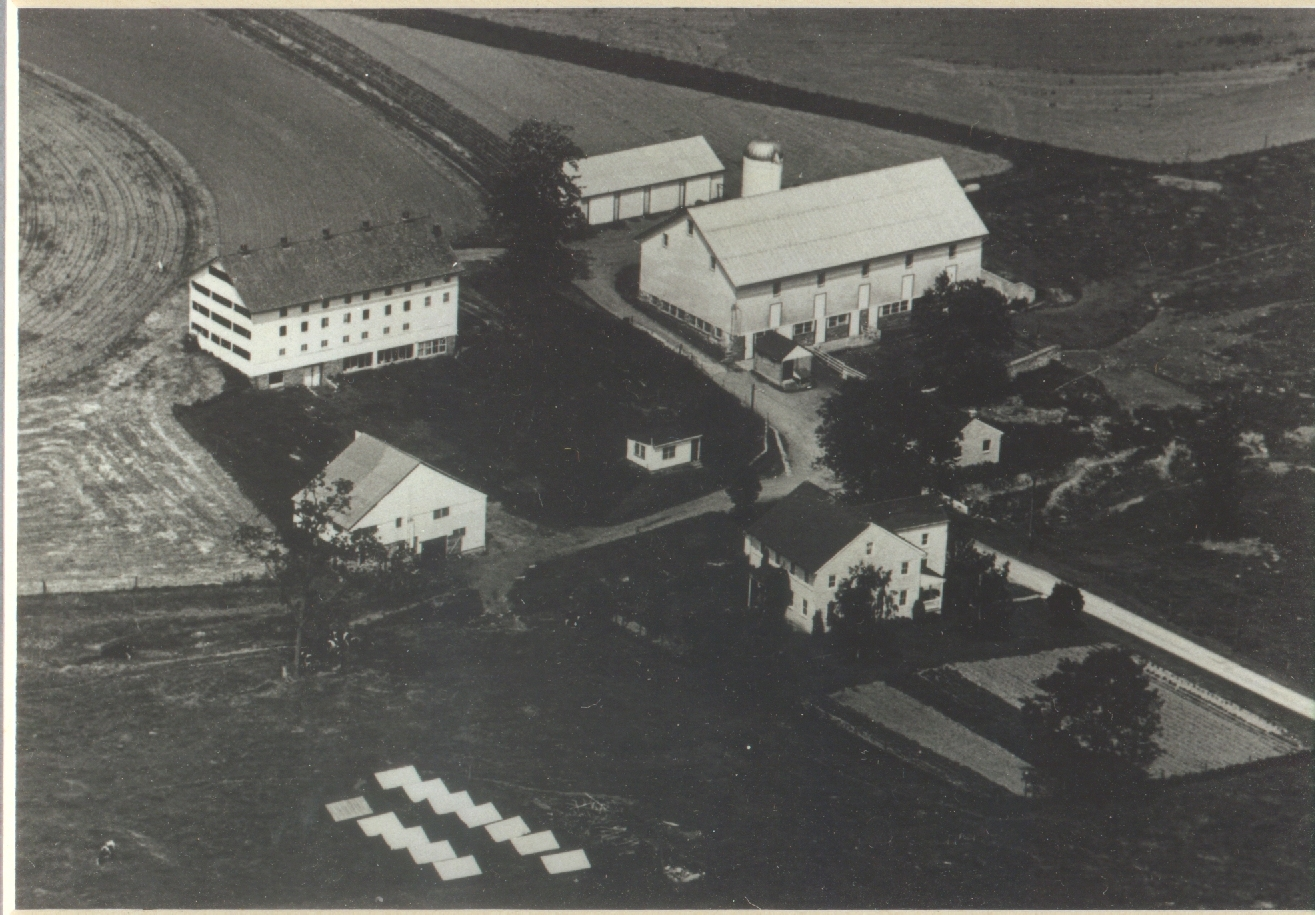
\includegraphics[width=0.9\textwidth]{my_family/7.jpg}
\caption{Grandma Hess, guests, and siblings 1963}
\label{grandma-hess}
\end{figure}

My face is hidden in this picture (Figure \ref{grandma-hess}) and that might reflect how I was feeling.
I was likely nine years old and not too happy about the way I had to dress.
Donna and Wayne, the two black children came to stay with us for two weeks through the Fresh Air program.
Donna was from Philadelphia and stayed with Grandma.
She came for several summers and kept in contact with Grandma into adulthood.
I believe that Wayne came from the city of York.
I believe he was only with us for one summer.
Grandma wanted to help where and when she could.
I have memories of my Papa driving to her house and bringing her to the farm to help my mother for at least one morning a week.
One of the jobs I remember her doing was ironing my father's dress shirts.
The collars of my father's shirts were starched stiff and were likely more time consuming than my mother had patience for.
There were a few times I remember staying with Grandma but it did not happen very often since older brothers and sisters were built in babysitters.

\begin{figure}
\centering
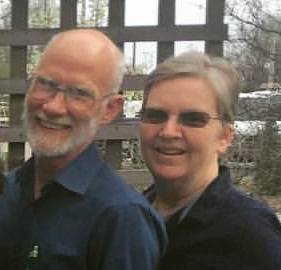
\includegraphics[width=0.8\textwidth]{my_family/8.jpg}
\caption{Christian and Mary Hess}
\label{christian-mary-hess}
\end{figure}

The story that I learned about Grandma and Grandpa (Christian) Hess as a young adult was one that I'm sure shaped who she was as an adult. Here is how I told the story.

The one grandmother that I knew was a widow for 60 years.
As a young person I wondered why my grandmother, Mary never remarried and as an adult learned the following story.
Mary's father Emanuel owned several farms and Christian and Mary were in the process of moving on to one of them with the goal of owning it one day when Christian died rather suddenly.
Mary was left with two young children, Verna (4 years old) and my father Jacob (1 year old).
What would happen to their plan? The story goes that Emanuel told his daughter Mary that if she married again he would not save the farm for his grandson, Jacob (my father), but if she chose to not marry again he would make sure the farm was available for him.
So the farm was rented to others while Mary moved home with her children.
From that home base she went out to care for other people's families when a baby was born.
She saw her children on the weekends and Verna and Jacob grew up under the watchful eye of their grandparents and later an uncle and aunt.


So what was this man, my Grandpa Hess like who drove himself to the doctor and heard the doctor tell him there was something wrong with his heart and he had only a short time to live? He drove home to give his young wife the news and died the day before his 29th birthday.
That is about all that I know of my Grandpa Hess.
My father had no stories to tell because he was not yet two years old when his father died and Grandma Hess did not tell stories easily.

Now to my mother's parents, Grandma (Cora) and Grandpa (Willis) Stauffer who I never met face to face. Grandpa Stauffer died on January 30, 1932 in the Lancaster General Hospital of pneumonia. Here is his obituary published in the Gospel Herald \footnote{GOSPEL HERALD - Vol. XXIV, No. 47 - February 18, 1932 - Page 1023}
\begin{quotation}
STAUFFER--WILLIS K. STAUFFER was born Aug. 15, 1895; died Jan. 30, 1932, at the Lancaster, Pa., General Hospital, from pneumonia. He was a faithful member of the Mennonite Church from early manhood. His place in the church was never vacant when health permitted. He was the son of Bro. and Sister Jacob N. Stauffer, deacon of the Masonville Church. Nov. 6, 1917, he was united in marriage to Sister Cora E. Warfel. To this union were born 2 sons and 6 daughters. One daughter preceded him in death. His loving companion remains to mourn his departure, with the following children: Mary W., Dorothy W., Anna W., Ethel W., H. Wilmer, J. Marvin, and Erma Mae. The family keenly feels the loss of a faithful companion and kind and loving father; the Church, a faithful member and teacher of the Bible Class. Funeral services were conducted Feb. 2 at the home, and at the River Corner, Pa., Mennonite Church, by Bros. Maris Hess, John H. Mosemann, and John K. Charles.

"Friends may think we have forgotten,

When at times they see us smile;

But they little know the heartache,

That is hidden all the while."

\end{quotation}

\begin{figure}
\centering
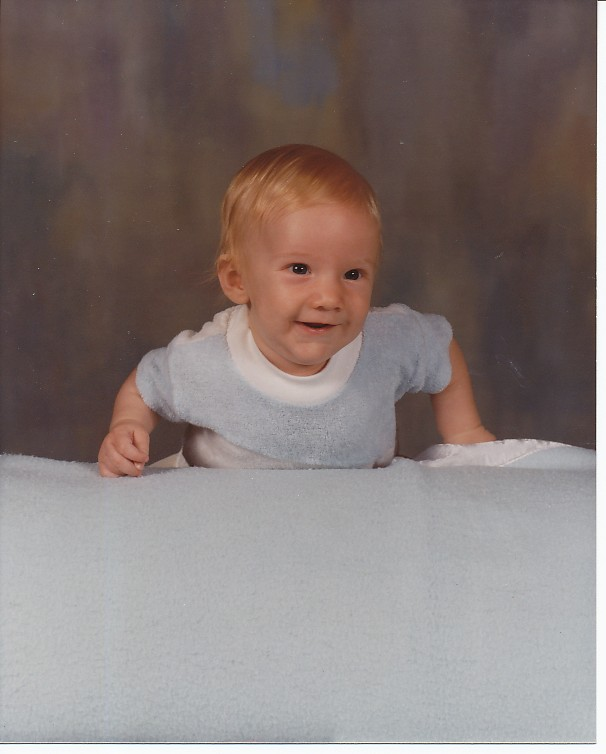
\includegraphics[width=0.8\textwidth]{my_family/9.jpg}
\caption{Willis and Cora Stauffer}
\label{willis-cora-stauffer}
\end{figure}

My mother was 12 at the time that her father died. 
It seemed to me that she always had a special place in her heart for her father. 
What little I've learned about him it seems he was a man with a plan.
He was going to buy a farm and raise vegetables for market.
This would keep his family of 7 living children busy.
But this was not to be. His youngest child, Erma was not yet a year old when he died. 

Cora seems to have been a determined and resourceful person. She would find a way to raise her family of children. She made potato chips and my mother told of selling bags of them on the streets of Conestoga the small town where they lived.
My mother enjoyed school and did well. 
So when it became financially necessary to have Mary leave school at the age of 16 and go to work on a farm, the school superintendent visited Grandma Cora with the goal of changing her mind. 
That was not possible and so Mary never finished high school. 
Instead she lived and worked on the farm of Aaron and Faith Shenk.

My Grandma Cora moved her family to share the farm house when Mary and Jacob started farming near New Danville.
They were planning to buy a house in Lancaster near Bridgeport along the Old Philadelphia Pike.
However Grandma Cora went to the hospital for a hysterectomy.
The next day she had a procedure done on the veins in her legs.
My parents visited her in the hospital and she was making a good recovery.
They returned to the work on the farm.
Only when they reached home there was a message that Grandma Cora had died of a pulmonary embolism (blood clot to the lungs).
I've been left with the understanding that someone made an error and Grandma Cora should not have died.
This was July 14, 1944.
Cora's youngest child was 13 years old and her oldest, my mother had three small children. 
The oldest was 2 years old. 
I'm sure Cora was greatly missed.

Here is her obituary published in the Gospel Herald\footnote{Gospel Herald Vol 37 \#21; 25 Aug 1944 pp 423-4}
\begin{quotation}
Stauffer.-Cora E. Stauffer, daughter of the late Hiram G. and Anna Mary (Sensing) Warfel, was born Nov. 6, 1894, in Conestoga Twp., Lancaster Co., Pa.; passed away in the Lancaster General Hospital, July 14, 1944; aged 49 y. 8 m. 8 d. Death was caused by a pulmonary embolism following a major operation 2 days before death. In early girlhood she accepted Christ as her personal Saviour and united with the River Corner Mennonite Church, remaining a faithful member until death. Her husband, Willis K. Stauffer, preceded her in death 12 years ago. She leaves to mourn her departure 2 sons and 5 daughters (Mary, wife of Jacob G. Hess, New Danville, Pa.; Dorothy W., Anna W., Ethel W., H. Wilmer, J. Marvin, and Erma Mae, all at home), 2 sisters (Mrs. Mary Shertzer, Farmersville, Pa., and Anna, wife of Chester Neff, Millersville, Pa.), a step-mother (Mary Warfel, Lancaster), and 3 grandchildren. One daughter (Edna) preceded her in death. Funeral services were held from her late home near New Danville, July 17, in charge of Bro. Maris Hess, and at the River Corner Mennonite Church, in charge of Bro. John K. Charles, assisted by Bros. Henry Nauman and James Hess. Burial was made in the adjoining cemetery.

Children: Edna W. Stauffer (1918 - 1923), Mary W Stauffer Hess (1920 - 2008), Dorothy W. Stauffer (1921 - 2004), Anna W Stauffer (1923 - 2010), Ethel W Stauffer (1924 - 2010), Jacob Marvin Stauffer (1930 - 2003), Erma Mae Stauffer Hunsberger (1931 - 2003)
\end{quotation}
